\documentclass{standalone}
\usepackage{tikz}
\usepackage{nono}
\begin{document}
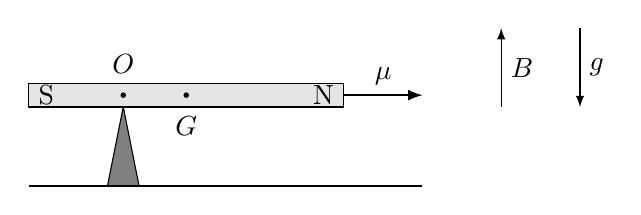
\begin{tikzpicture} 
  \draw[thick] (0,0) -- (5,0);
  \draw[fill=gray] (1, 0) -- ++(0.2, 1) -- ++(0.2, -1) -- cycle; 
  \draw[fill=gray!20] (0,1) rectangle ++(4, 0.3);
  \draw (1.2, 1.15) node[above=0.15cm]{$O$}; 
  \draw (2, 1.15) node[below=0.15cm]{$G$}; 
  %\draw[<->] (0, 1.7) -- (4, 1.7) node[midway, fill=white]{$L$}; 
  \fill (2, 1.15) circle (1pt);
  \fill (1.2, 1.15) circle (1pt);
  \draw (4, 1.15) node[left]{N};
  \draw (0, 1.15) node[right]{S};
  \draw[thick, -latex] (4, 1.15) -- ++(1,0) node[midway, above]{$\vv{\mu}$}; 

  \draw[-latex] (6, 1) -- ++(0, 1) node[midway, right]{$\vv{B}$};  
  \draw[-latex] (7, 2) -- ++(0, -1) node[midway, right]{$\vv{g}$};  
\end{tikzpicture}
\end{document}
